\documentclass[a4paper,12pt]{article}

\usepackage[a4paper, margin=1in]{geometry}
\usepackage[ruled]{algorithm2e}
\SetKwInOut{Input}{Input}\SetKwInOut{Output}{Output}
\usepackage{algpseudocode}
\usepackage{amsfonts}
\usepackage{amsmath}
\usepackage{amssymb}
\usepackage{xspace}
\usepackage{xcolor}
\usepackage{setspace}
\usepackage{lineno}
\usepackage{outlines}
\usepackage[normalem]{ulem}
\usepackage{paralist}
\usepackage{graphicx}
\usepackage{caption}
\usepackage{subcaption}
\usepackage{url}


\newcommand{\prob}{\ensuremath{\mathrm{Pr}}}
\newcommand{\dB}{de~Bruijn\xspace}
\newcommand{\dBG}{de~Bruijn graph\xspace}
\newcommand{\dBCM}{DBCM\xspace}
\newcommand{\dBHT}{DBHT\xspace}
\newcommand{\cm}{CountMin\xspace}
\newcommand{\kmer}{\mbox{$k$-mer}\xspace}
\newcommand{\kmers}{\mbox{$k$-mers}\xspace}
\newcommand{\chr}[1]{\ensuremath{\mathtt{#1}}}
\newcommand{\A}{\chr{A}}
\newcommand{\C}{\chr{C}}
\newcommand{\G}{\chr{G}}
\newcommand{\T}{\chr{T}}
\newcommand{\keyterm}[1]{\textit{#1}\/\xspace}
\newcommand{\str}[2]{\ensuremath{#1_0\cdots#1_{#2-1}}}
\newcommand{\strname}[1]{\ensuremath{\uppercase{#1}}}
\newcommand{\strdef}[2]{\ensuremath{\strname{#1}=\str{#1}{#2}}}
\newcommand{\strslice}[3]{\ensuremath{\strname{#1}[#2:#3]}}
\newcommand{\strsetname}[1]{\ensuremath{\mathcal{\uppercase{#1}}}}
\newcommand{\mega}{\ensuremath{\mathrm{M}}}
\newcommand{\kilo}{\ensuremath{\mathrm{K}}}

\newcommand{\todo}[2][]{\color{red} [#1] #2 \color{black}}
\newcommand{\tochange}[1]{\color{red} #1 \color{black}}
\newcommand{\toconsider}[1]{\color{blue} #1 \color{black}}
\newcommand{\changed}[1]{#1}%{\color{teal} #1 \color{black}}
\newcommand{\asq}[1]{\color{red}$\rightarrow$ asq says: #1 $\leftarrow$ \color{black}}
\newcommand{\paguso}[1]{\color{magenta}$\rightarrow$ paguso says: #1 $\leftarrow$ \color{black}}
\newcommand{\remove}[2][]{\color{magenta}{\sout{#2}(\textit{#1})}\color{black}}
\newcommand{\change}[3][]{\remove[#1]{#2}{#3}}
\newcommand{\readset}{\strsetname{X}\xspace}


\title{Space-efficient representation of \dBG{s} for sequence data streams}
\author{Augusto Queiroz, Nivan Ferreira, Paulo Fonseca}

\begin{document}
	
\maketitle

\begin{abstract}
\noindent\textbf{Background} A \dBG represents a given set of sequencing reads by the corresponding set of distinct \kmers, taking into account their overlaps, and have been used extensively for biological sequence assembly and analysis since the advent of second-generation sequencing technologies. However their construction time and memory cost remain two major bottlenecks, especially in the presence of sequencing errors.

\noindent\textbf{Objectives} Our aim is to develop a \dBG representation that faithfully represents the \kmers in the reads, while leaving out spurious fragments due to sequencing errors. Not only we want our representation to have a good sensitivity to specificity ratio, but we also want it to be space and time-efficient in practice.

\noindent\textbf{Methods} We propose a pipeline to build a navigational \dBG data structure using two consecutive probabilistic representations based on a \cm sketch and a hashtable. This pipeline filters \kmer{s} on the basis of frequency and connectivity to other \kmer{s}, representing only high-quality \kmer{s} in a succinct manner. It is suited for sequence reads fed as a data stream, dispensing with the usual preprocessing step of counting distinct \kmers. 

\noindent\textbf{Results} We applied our method to \todo{real data} showing that it effectively filters-out \todo{over $80\%$} of spurious \kmer{s} based on frequency alone, and \todo{over $95\%$} of them in total using the connectivity-based traversal filter. Our representation ultimately requires between \todo{$9$ and $16$~bits} per \kmer, while allowing for constant time insertion and query. We show that even with \todo{$9$} bits per \kmer, the number of false positive \kmer{s} is still \todo{less than $16\%$} of the total graph. \todo{How about contigs?}

\noindent\textbf{Conclusion} The proposed pipeline uses connectivity-based filtering of \kmers through \dBG traversal very effectively, leading to a streamlined data structure \todo{more conclusions}.

\end{abstract}

	
\section{Introduction}

\section{Methods}

The \keyterm{\dBG} (dBG) of order $k$ of a string \strdef{x}{n}, $G(X;k)=(V,E)$, is defined as the directed graph whose nodes $V$ represent all distinct \kmer{s} (i.e. substrings of length $k$) of \strname{X}, and such that any two nodes representing $(k-1)$-overlapping \kmer{s} are connected by an edge labeled by the last character of the second \kmer. For example if $k=3$ and $X$ contains the substring \chr{ACGT} then the consecutive triplets \chr{ACG} and \chr{CGT} originate the edge $\chr{ACG}\stackrel{\chr{T}}{\longrightarrow}\chr{CGT}$. Hence the edges $E$ represent all distinct $(k+1)$-mers of $X$. This definition  generalizes to a set of strings simply by taking all \kmers of all sequences in the set.
% That is, given two nodes on the graph, they each represent a distinct sequence of symbols $S_1$ and $S_2$, and there is an edge between them if and only if the tail of $S_1$ is the head of $S_2$.
In genome sequencing, dBGs are used to represent the distinct \kmer{s} in a set \readset of \keyterm{reads} generated by the sequencer, which correspond to randomly distributed fragments of the source DNA \strname{S}. The amount and total length of the reads is determined by the \keyterm{coverage} or \keyterm{depth}, which is the average number of reads containing each base in \strname{S}. 
%Ideally, \strname{S} could be obtained from an Eulerian traversal of $G(\readset, k)$. Unfortunately however, due to sequencing errors and repeats, such a straightforward approach is not feasible, but the \dBG can still be used to produce a collection of partial assemblies, called \keyterm{contigs}, which can then be further combined to form the original genome \cite{Pevzner2001}. Figure~\ref{fig:dbgexample} presents an example of the \dBG in this context.

\begin{figure}[htbp]
	\begin{center}
	%	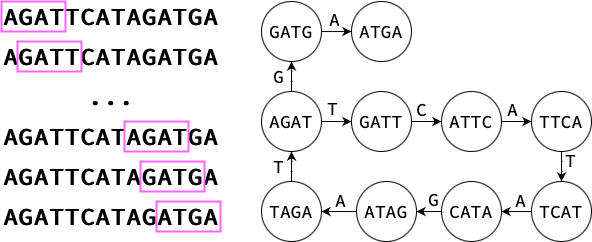
\includegraphics[width=0.8\textwidth]{figures/dbg-example}
	\end{center}
	\caption{Example of a \dBG. $k=4$}\label{fig:dbgexample}
\end{figure}

%\section{Reverse Complements}
%\label{subsec:dBG-reversecomplements}

One difficulty of using dBGs to represent DNA is the presence of \keyterm{reverse complements}. The sequencer reproduces either of the two complementary strands of any input fragment, such that the output read may correspond to the sequence \strname{X} in the forward (5'-3') direction, or its reverse complement \strname{\overline{X}} in the backward (3'-5') direction.
%, with\strname{\overline{S}} being obtained from \strname{S} by swapping each base with its Watson-Crick complement ($\A \leftrightarrow \T$, $\C \leftrightarrow \G$) and then reversing the string, and vice versa. For example, the reverse complement of the sequence $S=\chr{AGTACGGTC}$ is $\overline{S}=\chr{GACCGTACT}$ and vice versa.
To deal with that, reads are usually processed twice, once in each direction,
%Nodes representing \kmer{s} that are reverse complements of each other are merged, and edges are made bidirectional. Alternatively, nodes are kept distinct
resulting in a symmetric graph in which ``a forward traversal corresponds to the backwards traversal on the reverse complement path, and vice versa.'' \cite{Conway2011}
% As in \cite{Conway2011}, this will be treated by processing
% all reads in both directions, without, however, merging nodes representing reverse complements. As noted by Conway \& Bromage: ``This
% makes the graph symmetric; a forward traversal corresponds to a backwards traversal on the reverse complement path, and vice versa.``
% \cite{Conway2011}

We propose two probabilistic navigational data structures \cite{Chikhi2014} for the dBG with node/edge membership queries that enable graph traversal. The first is based on the \cm sketch \cite{Cormode2005} and is constructed directly from the reads, without preprocessing, in an online fashion, so that the sequences may be given as a data stream. It performs online \kmer counting and can also be traversed through the use of a probabilistic neighborhood query in a space-efficient manner. We call this structure the \keyterm{\dB \cm}, or \dBCM for short. The second structure is a hashtable-based representation called \keyterm{\dB hashtable}, or \dBHT, built from the \dBCM for improved time and space-efficiency. Both structures are designed to facilitate graph navigation by storing a set of outgoing edges (outedges, for short) together with each \kmer, allowing for constant time neighborhood queries. 

%These two structures can be used in tandem to leverage the benefits of each one individually. We construct the \dBCM directly from the reads, without preprocessing, such that the reads can be treated as a data stream and added into the structure as soon as they are made available. During processing, we store in disk a set of possible starting \kmer{s} \strsetname{S} taken from the reads. Once all the reads have been processed, we traverse the \dBCM starting from the \kmer{s} in \strsetname{S}, inserting the visited nodes and their outedges into a \dBHT. This pipeline can be seen in Algorithm~\ref{alg:pipeline}.

\todo[mover para logo antes de introduzir DBHT]{Because spurious \kmer{s} happen in sequence (e.g. a single erroneous base is likely to cause the $k$ \kmer{s} that include it to become erroneous), they create branches off of the graph generated by the real \kmer{s}. If a single \kmer of such a branch is identified as spurious and not included in the graph, however, it causes all subsequent \kmer{s} to be unreachable through traversal. As such, \kmer{s} that would be included in the \dBG based on frequency alone may be excluded when constructing the \dBHT from traversal due to a predecessor being correctly filtered out.}

%\begin{algorithm}
%	\caption{Pipeline}\label{alg:pipeline}
%	\Input{\readset, a set of sequencing reads; $t$, the frequency threshold for a \kmer to be considered true; $n$ the number of starting \kmer{s} for traversal to take from the reads}
%	\Output{The \dBHT representation of the \dBG}
%	$C \gets$ an empty \dBCM\\
%	$\strsetname{S} \gets C.\mathit{construct}(\readset, t)$\Comment{see Section~\ref{subsubsec:dbcm-construction}}\\
%	$T \gets$ an empty \dBHT\\
%	$T.\mathit{construct}(C)$\Comment{see Section~\ref{subsubsec:dbht-construction}}\\
%	\Return{$T$}
%\end{algorithm}


\subsection{The \dBCM sketch}
\label{sec:debruijncountmin}

%In order to leverage the benefits of an NDS in reducing the impact of the false positive rate of the membership operation, we introduce a modified version of the original \cm sketch, presented below, called \keyterm{\dB\cm} (\dBCM) allowing for querying not only for \kmer counts, but also for the outedges from the corresponding nodes in the \dBG. As such, the \dBCM implements not only a membership query operation as detailed in Section~\ref{subsubsec:cm-dbg}, but also a neighborhood query.


%\subsection{The \cm sketch}
%\label{sec:countmin}

The DBCM is an adaptation of the \cm sketch \cite{Cormode2005}, which is a sublinear data structure for event frequency estimation
%. Given a stream of events $\strsetname{X} = \{(x_i, c_i) | i \in \mathbb{N}\}$, where $c_i \geq 0$ is the number of occurrences of $x_i$, it offers 
with two basic operations, $update(x, n)$ and $count(x)$, respectively for informing $n$ occurrences of an event $x$, and for estimating the accumulated number of occurrences of event $x$ up to that point.
It consists in a $d\times w$ matrix of counters $C$, coupled with a set of $d$ pairwise-independent hash functions $h_0\ldots h_{d-1}$. The $update(x,n)$ operation uses $h_i$ to map $x$ to one of the $w$ cells in each row $i$, and then increments the counter $C[i,h_i(x)]$ by $n$. 
%Here we consider only individual event occurrences, so that counters are always incremented by one.
The $count(x)$ query gets the values of the counters associated with the event $x$ in each row $i$,  and then returns their minimum, that is $count(x)=\min\{C[i,h_i(x)]; i=0\ldots d-1$\}.
%Figure \ref{fig:countminexample} presents a visualization of the \cm sketch.

% \begin{figure}[htbp]
% 	\begin{center}
% 		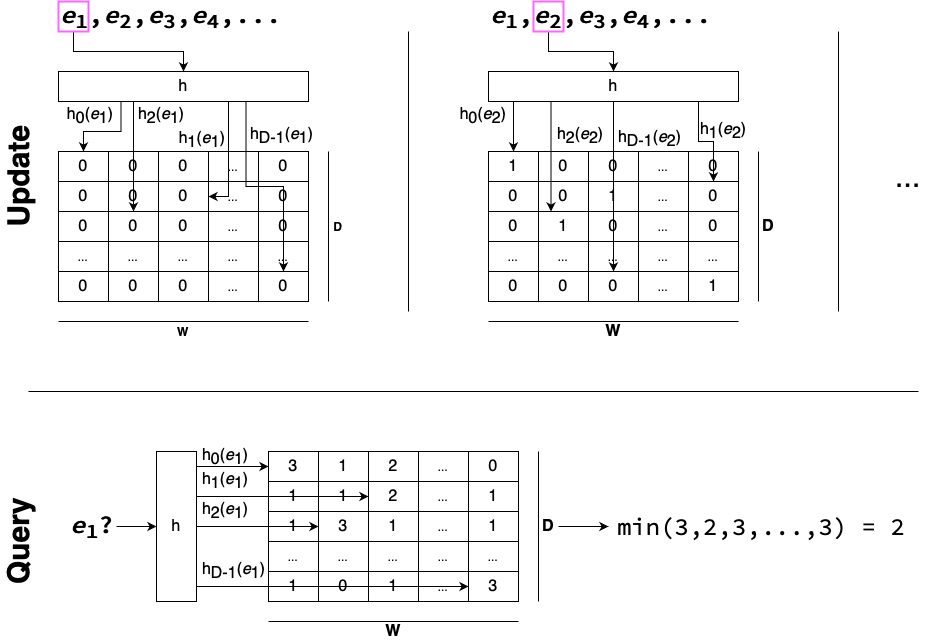
\includegraphics[width=0.9\textwidth]{figures/cm-example}
% 	\end{center}
% 	\caption{Example of a \cm sketch}\label{fig:countminexample}
% \end{figure}

The \cm might overestimate the frequency of a given event due to hash collisions. However, by setting large enough $w$ and $d$, we can control for the probability of collisions, and hence the estimation accuracy. More specifically, given two parameters $\epsilon, \delta \in (0,1)$, by setting 
$w=O(2/\epsilon)$ and $d=O(\log1/\delta)$, we have
\begin{equation}
\label{eq:cm-prob}
%\prob[C.\mathit{query}(x) - c(x) > \epsilon \|\strsetname{X}\|_1] < \delta,
\prob[count(x) - N(x) > \epsilon N] < \delta,
\end{equation}
where $N(x)$ represents the true count of event $x$,
%, \strsetname{X} is the set of all events, and $\|\strsetname{X}\|_1=\sum_{x_i\in\strsetname{X}}c(x_i)$ 
and $N=\sum_x N(x)$ stands for the total event count. This means that the estimation error relative to the total event count can be made `small' (no more than $\epsilon$) with `good' (at least $1-\delta$) probability.


%Zhang \emph{et al.} proposed using a \cm sketch to count \kmer{s} \cite{Zhang2014}. 
The DBCM adapts and extends a \cm to represent a dBG as it is built from a set of reads. As mentioned before, we process reads as a stream of sequences, taking each \kmer in the forward and backward direction as an event. Technically, we treat each \kmer as a base-4 $k$-digit integer, with $\A=0$, $\C=1$, $\G=2$, $\T=3$. 
%For example, the \kmer $\C\G\A\T\A$ can be interpreted as the integer $12030_{(4)} = 396_{(10)}$. 
%Whenever we refer to hashing a \kmer, we use its integer interpretation. 
\todo[do we need this info?]{Using a \cm introduces the chance that any reported count will be an overestimate, the probability of which is approximately $(1-e^{-N/w})^d$, with $N$ the number of distinct \kmer{s} \cite{Zhang2014}}.

We decide whether or not to consider a \kmer $x$ as a dBG vertex based on its count, the idea being that a true \kmer should be read a number of times close to the sequencing coverage, whereas a spurious \kmer should appear much less frequently in comparison. 
Hence the DBCM node membership operation considers a \kmer to be represented in the graph iff $count(x) \geq t$ for some threshold $t$ related to the coverage. 
Assuming that the vast majority of low-frequency \kmers occur no more than once or twice in the input reads, in order for such a \kmer to be unduly considered as real (false positive), its count estimate would have to be off by about $t$ or more. Because the overestimation error is at most $\epsilon N$ with probability at least $1-\delta$, according to \eqref{eq:cm-prob}, by setting this maximum error to $\epsilon N=t$, we have that the expected false positive rate is no more than $\delta$. This amounts to setting the matrix dimensions to $w=O(2/\epsilon) = O(2N/t)$ and $d=O(\log 1/\delta$).


%As the count returned by the \cm sketch can be overestimated by some error $\epsilon F$ with probability $\delta$ as established in Equation~\ref{eq:cm-prob}, we can arrive at an expression for the probability that a low-frequency \kmer will be considered to be a member of the \dBG by defining $\epsilon F = t$. This takes into account that most spurious \kmer{s} appear only once or twice in the reads, as discussed in Section~\ref{subsec:dBG-selectingkmers}. Due to the relationships between $w$ and $\epsilon$, and $d$ and $\delta$, we can decide the necessary size of the \cm sketch to achieve the desired false positive rate by making $\delta$ the desired rate, choosing $d = \log \frac{1}{\delta}$, and making $w = \frac{2}{\epsilon} = \frac{2F}{t}$.


% - Representation (what goes in each cell)
% - Operations:
%   - addOutEdge
%   - query 
% - Analysis space/time (may be done within previous sections)

% Because we expect each \kmer from the sequence to appear in the reads a number of times equals to the coverage, while spurious \kmer{s} will appear a low number of times \cite{Conway2011} \cite{Ghosh2019}, a structure used to count \kmer{s} (that implements the $\mathit{count}(x)$) can implement the membership query operation as $\mathit{memb}(x)=\mathit{count}(x) \geq t$. In this way, a \cm sketch can \toconsider{probabilistically} represent a \dBG with some false positive and false negative rates associated with the membership query operation. These rates can be controlled by $t$.\asq{Aqui talvez valha a pena falar que existem duas abordagens para tentar controlar as taxas de falsos positivos e negativos: 1. O valor de $t$ pode ser estabelecido, e, então, os valores de $w$ e $d$ são calculados de forma a minimizar a chance de um erro $\epsilon > t$; 2. Os valores $w$ e $d$ podem ser fixados, e, então, $t$ é decidido baseado nas estimativas esperadas para um \kmer espúrio \emph{vs.} um \kmer real.}

% Selecting the appropriate value for $t$ is not a trivial task, however, and is a trade-off between the false positive and false negative rates. Due to the fact that reads are generated randomly from the original genome, and that a number of real \kmer{s} will be replaced by spurious \kmer{s} because of sequencing errors, an universally optimal threshold \toconsider{that perfectly decides if a \kmer is spurious or not} does not exist. Higher values of $t$ are more likely to cut out spurious \kmer{s}, reducing false positive rates, but they also increase the chances of a real \kmer being missed, increasing false negative rates. Lower values of $t$ result in the opposite effect happening.

%\subsection{\cm as a probabilistic NDS representation for \dBG{s}}
%\label{subsubsec:cm-dbg}

In order to make the representation more easily navigable, we augment the data structure such that each cell $[i,j]$ in the matrix stores not only the counter $C[i,j]$, but also a set of outedges $E[i,j]$. The DBCM then provides an operation $add\_outedge(x,a)$ to add an outgoing edge to the node/\kmer $x$ with label $a\in\{\A,\C,\G,\T\}$, and an operation $outedges(x)$ that returns the set of outedges of the \kmer node $x$. The latter is also called `\emph{outneighborhood}' or `star' operation. \todo[Isso é feito assim?]{An individual edge membership query can be derived from the node membership and star operations.}

%The update operation is the same as in a regular \cm, and the procedure for adding an edge can be seen in Algorithm~\ref{alg:addOutEdge}.
The $add\_outedge(x,a)$ operation works similarly to a count update, except that it adds $a$ to the sets $E[i,h_i(x)]$ for each row $i$. This means that the outedge $a$ must be represented in all cells associated to node $x$. On the other hand, hash collisions may cause unrelated edges to be added to some of those cells, but hopefully not all of them. Therefore the $outedges(x)$ operation returns the intersection of the sets of the cells associated with node $x$, that is $outedges(x)=\bigcap _i E[i,h_i(x)]$.  

%\begin{algorithm}[htbp]
%	\caption{$C.\mathit{add\_outedge}(X, a)$}\label{alg:addOutEdge}
%	\Input{C, the \dBCM; $X$, the \kmer; $a \in \{\A, \C, \G, \T\}$, the outedge label}
%	\For{$i \gets 0, \ldots, d-1$}{
%		$C[i,h_i(X)].E \gets C[i,h_i(X)].E \cup \{a\}$\\
%	}
%\end{algorithm}

%Besides the query operation, used for obtaining the count for a given \kmer $X$, done in the same way as in a regular \cm, the \dBCM must also implement an operation for retrieving the outedges for $X$. This new operation is presented in Algorithm~\ref{alg:dbcm-outedges}.

% \begin{algorithm}
% 	\caption{$C.\mathit{outedges}(X)$}\label{alg:dbcm-outedges}
% 	\Input{$C$, the \dBCM; $X$, the \kmer}
% 	\Output{The outedge set $E$}
% 	$E \gets \{\A, \C, \G, \T\}$\\
% 	\For{$i = 1, \ldots, d$}{
% 		$E \gets E \cap C[i,h_i(X)].E$\\
% 	}
% 	\Return{$E$}
% \end{algorithm}

In practice, due to a node having at most four outedges (labeled \A, \C, \G, or \T), we can represent them with four indicator bits. An edge is added by setting the corresponding bit in each cell, and their intersection is obtained by performing bitwise AND operations. Moreover the set of outedges $E[i,j]$ and the counter $C[i,j]$ are packed together in a single 16-bit integer. 
%This layout can be visualized in Figure~\ref{fig:dbcm-bit_use}. 
Assuming that we use a large enough $k$ such that each \kmer is expected to appear no more than a few times in the original sequence $S$, and hence a number of times approximately equal to the coverage $c$ in the reads, and considering also that $c$ is not a very high value (commonly $\leq 200$), 12-bit counters should suffice to account for the expected counts of all real \kmers, as well as possible collisions.

% \begin{figure}[htbp]
% 	\centering
% 	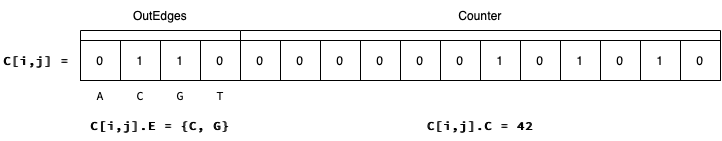
\includegraphics[width=0.9\textwidth]{figures/dbcm-bit_use}
% 	\caption{A \dBCM cell}\label{fig:dbcm-bit_use}
% \end{figure}

\subsubsection{\dBCM Construction}
\label{subsubsec:dbcm-construction}

The \dBCM is constructed as the reads are processed by incrementing the counters for each \kmer in both directions. Once a \kmer counter reaches the threshold $t$, an outedge is added from the preceding \kmer to the current one. That is, for two consecutive \kmers $x$ and $y$, if $\mathit{count}(y) \geq t$, then $\mathit{add\_outedge}(x, y[k-1])$ is performed, where $y[k-1]$ denotes the last character of $y$. 

Notice that, in order to add an edge from $x$ to $y$, we require only $y$ to be of high-frequency. Indeed, if $y$ were not be represented in the final graph, such an edge would at best result in unnecessary operations. In the worst case it could be interpreted, due to a collision, as a diferent edge, resulting in a new spurious branch on the graph. Conversely, adding an outedge from a low count \kmer $x$ is less harmful, since it will be ignored in the final graph and the edge will not be considered for traversal. We also avoid the scenario where both $x$ and $y$ are real \kmers, but $y$ shows up for the last time before $x$ is considered to be present, in which case this real edge would be ommited. 

Finally, the construction step also compiles a set $\strsetname{S}$ of true \kmers that can be used as starting points for graph traversal. 
%\todo{Quem são esses nós? Como são escolhidos, onde são gravados?}. 
Ideally, only the first \kmer from the original sequence $S$ would be sufficient, but we have only the reads and ignore where they were taken from. So we consider instead the \kmers that are at the extremities of their reads in both directions, assuming that the following \kmers will be reachable from them.
\todo{Onde esse conjunto é gravado?}
%, as further discussed in Section~\ref{subsubsec:dbcm-navigation}. 

% The procedure for constructing a dBCM can be seen in Algorithm~\ref{alg:dbcm-construction}. Like Conway \& Bromage \cite{Conway2011}, we process each read in the forward and in the reverse complement direction, without merging \kmer{s} corresponding to reverse complements of each other.

% \begin{algorithm}
% 	\caption{$C.\mathit{construct}(\readset, t, n)$}\label{alg:dbcm-construction}
% 	\Input{$C$, the \dBCM; $\readset$, the set of reads; $t$, the frequency threshold for a \kmer to be considered true; $n$, the number of \kmer{s} from each read to be included in \strsetname{S}}
% 	\Output{\strsetname{S} the set of starting \kmer{s}}
% 	$C.t \gets t$\\
% 	$\strsetname{S} \gets \emptyset$\\
% 	$\overline{\readset} \gets \{\overline{R}; R \in \readset \}$\Comment{The set of the reverse complements of the reads}\\
% 	\For{$R \in \readset \cup \overline{\readset}$}{
% 		$X \gets \varnothing$\\
% 		$i \gets 0$\\
% 		\For{$Y \in \kmer{s}(R)$}{
% 			$C.\mathit{update}(Y)$\\
% 			\If(\Comment{see Section~\ref{subsubsec:dbcm-operations}}){$C.\mathit{is\_member}(Y)$}{
% 				\If{$i \leq n$} {
% 					$\strsetname{S} \gets \strsetname{S} \cup \{Y\}$\\
% 				}
% 				\If{$i > 0$}{
% 					$C.\mathit{add\_outedge}(X, Y[i-1])$\\
% 				}
% 			}
% 			$i \gets i+1$\\
% 			$X \gets Y$\\
% 		}
% 	}
% 	\Return{\strsetname{S}}
% \end{algorithm}

% \subsection{\dBCM Operations}
% \label{subsubsec:dbcm-operations}

% % We can implement the operations listed in Section~\ref{subsubsec:dbg-operations} using the \dBCM as follows.

% % \paragraph*{Membership query} Given the desired presence threshold $t$, we can implement the membership query operation in the \dBCM as $C.\mathit{is\_member}(X) \equiv C.\mathit{query}(X).c \geq C.t$.

% % \paragraph*{Forward neighbor query} $C.\mathit{forward\_neighbor}(X, a) \equiv a\in C.\mathit{query}(X).E$.

% % \paragraph*{Neighborhood query} We can transform the set of outedges $C[i,j].E$ into a set of \kmer{s} by extending the \kmer with the outedges from the set. As such, a procedure for generating the set of neighbors for a given \kmer $X$ is found in Algorithm~\ref{alg:dbcm-neighbors}.

% % \begin{algorithm}
% % 	\caption{$C.\mathit{neighbors}(X)$}\label{alg:dbcm-neighbors}
% % 	\Input{$C$, the \dBCM; $X$, a \kmer}
% % 	\Output{$N$, a set of \kmer{s} that are neighbors of $X$}
% % 	$N \gets \emptyset$\\
% % 	\For{$a \in C.\mathit{query}(X).E$}{
% % 		$N \gets N \cup \{X[1:k-1] \cdot a\}$\\
% % 	}
% % 	\Return{$N$}
% % \end{algorithm}

% % \subsection{\dBCM Traversal}
% % \label{subsubsec:dbcm-navigation}

% % This structure can be traversed in a breadth-first order from an initial set of \kmer{s} $\strsetname{S}$ by querying for their out-edges and then querying each of their neighbors, repeating this for each neighbor found to be in the graph. This procedure can be observed in Algorithm~\ref{alg:traversal}.

% % \begin{algorithm}
% % 	\caption{$C.\mathit{traverse}(\strsetname{S}, t)$}\label{alg:traversal}
% %   \Input{$C$, the \dBCM; $\strsetname{S}$, the set of starting \kmer{s}; $t$, the threshold of presence}
% %   \Output{$V$, the set of \kmer{s} queried from the \dBCM during traversal}
% %   $F \gets$ empty Queue\\
% %   \For{$s \in \strsetname{S}$}{
% %     enqueue($F$, $s$)\\
% %   }
% %   $V \gets \{\}$\\
% %   \While{$F$ is not empty} {
% %     $u \gets$ dequeue($F$)\\
% %     $V \gets V \cup \{u\}$\\
% %     $n, E \gets C.query(u)$\\
% %     \If{$n \geq t$}{
% %       \For{$a \in E$}{
% %         $v \gets$ extend($u$, $a$)\\
% %         \If{$v \notin V$}{
% %           enqueue($F$, $v$)\\
% %         }
% %       }
% %     }
% %   }
% % 	\Return{$V$}
% % \end{algorithm}

% \begin{algorithm}
% 	\caption{$C.\mathit{traverse}(\strsetname{S}, t)$}\label{alg:traversal}
% 	\Input{$C$, the \dBCM; $\strsetname{S}$, the set of starting \kmer{s}; $t$, the threshold of presence}
% 	\Output{$V$, the set of \kmer{s} queried from the \dBCM during traversal}
% 	$F \gets$ empty Queue\\
% 	\For{$s \in \strsetname{S}$}{
% 		enqueue($F$, $s$)\\
% 	}
% 	$Q \gets \{\}$\\
% 	\While{$F$ is not empty} {
% 		$u \gets$ dequeue($F$)\\
% 		$Q \gets Q \cup \{u\}$\\
% 		\If{$C.\mathit{is\_member}(u, t)$}{
% 			\For{$v \in C.\mathit{neighbors}(u)$}{
% 				\If{$v \notin Q$}{
% 					enqueue($F$, $v$)\\
% 				}
% 			}
% 		}
% 	}
% 	\Return{$Q$}
% \end{algorithm}

% \paragraph*{Selecting the starting set $\strsetname{S}$ of \kmer{s} for traversal} Ideally, only the first \kmer from the original sequence $S$ is needed to perform the traversal of the graph, but unfortunately it is not possible to determine where in the original sequence a read was taken from. One option is to use all the \kmer{s} from the reads that are found to be in the graph, but we argue that this set is unnecessarily large. We can instead reduce the size of $\strsetname{S}$ by only considering the \kmer{s} that are at the start of their reads since the following \kmers would be reachable from it anyway.

\subsection{The DBHT}
\label{sec:debruijnhashtable}
% - Structure
%   - fingerprint
%   - Outedges
% - Hash function 
% - Collision resolution
% - Operations 
%   - Add node/edge
%   - Query node/edge/star 
% - Analysis 

We also propose a new hashtable-based representation for the \dBG, called \keyterm{\dB Hashtable} \dBHT, that is made more space-efficient by not storing the \kmer directly. Instead, the slot $T[i]$ containing the \kmer $X$ stores a \keyterm{fingerprint} $T[i].f = f_X$, computed from $X$ as described in Section~\ref{sec:fingerprint}, along with the set of outgoing edges from $X$, $T[i].E$,  as described in Section~\ref{sec:debruijncountmin}.

When inserting a \kmer $X$ into a \dBHT of capacity $m$, a hash value $h_X$ and the fingerprint $f_X$ are calculated in parallel. The hash value, computed as described in Section~\ref{sec:fibhash}, determines the initial position $p_0$ in which the \kmer should be stored. If this slot is empty, then the fingerprint is written there. Otherwise, collisions are resolved by linear probing, that is the subsequent positions $(p_0+j)\mod m$, for $j=0\ldots m-1$, are checked until a free slot is found. If, however, a slot containing $f_X$ is found before, then $X$ is considered to be already represented in $H$ and the insertion aborts. This process is detailed in Algorithm~\ref{alg:ht-insert}. 
Notice that this requires always having some unused slots, that is, having a \emph{load factor} $0 < \alpha=n/m < 1$, where $n$ is the number of used positions. Higher values of $\alpha$ will result in higher space-efficiency, but also` more collisions. Lower values have the opposite effect. 


\begin{algorithm}
	\caption{$T.\mathit{insert}(X$)}\label{alg:ht-insert}
	\Input{$T$: a \dBHT with capacity $m$; $X$: the \kmer to be inserted}
	$h_X \gets \mathit{fibhash}(X, m)$\Comment{see Section~\ref{sec:fibhash}}\\
	$f_X \gets \mathit{fingerprint}(X)$\Comment{see Section~\ref{sec:fingerprint}}\\
	$i \gets h_X$\\
	\While{$T[i]$ is not empty}{
		\eIf{$T[i].f = f_X$}{
			\Return{}\Comment{$X$ already in $T$}
		}{
			$i \gets (i + 1)\mod m$\\
		}
	}
	$T[i].f\gets f_X$\\
	$T[i].E\gets \varnothing$\\
\end{algorithm}

To query the hashtable for a \kmer/node $X$, the same sequence of positions as in the insertion are probed until the desired fingerprint $f_X$ is found, or a free position is reached, in which case we can conclude that the \kmer is absent from the structure. This operation is presented in Algorithm \ref{alg:ht-query}.

\begin{algorithm}
	\caption{$T.\mathit{query}(X)$}\label{alg:ht-query}
	\Input{$T$: a \dBHT with capacity $m$; $X$: the \kmer to be queried}
	$h_X \gets \mathit{fibhash}(X, m)$\\
	$f_X \gets \mathit{fingerprint}(X)$\\
	$i \gets h_X$\\
	\While{$T[i]$ is not empty}{
		\eIf{$T[i].f = f_X$}{
			\Return{$T[i].E$}
		}{
			$i \gets (i + 1) \mod m$\\
		}
	}
	\Return{$\varnothing$}
\end{algorithm}


Adding an edge $X\stackrel{a}{\longrightarrow}Y$ to the \dBHT is similar to adding a \kmer node, and breaks down to, first, locating the slot $T[i]$ of the source node $X$, and then adding the corresponding edge label $a$ to its set of outedges. As before, this is done by setting the appropriate bit of the  4-bit pattern $T[i].E$. This procedure is detailed in Algorithm~\ref{alg:ht-addedge}. Note that, because two \kmer{s} can be mapped to the same cell, the outedges stored for both of them will be the same and will contain the true outedges of each one individually. This further makes it important that edges only be added to nodes known to be in the graph, which the \dBHT does not verify.


\begin{algorithm}
	\caption{$T.\mathit{add\_outedge}(X, a)$}\label{alg:ht-addedge}
	\Input{$T$: a \dBHT with capacity $m$; $X \in \{\A, \C, \G, \T\}^k$: the \kmer to be queried; $a \in \{\A, \C, \G, \T\}$: the edge label to be added}
	$h_X \gets \mathit{fibhash}(X, m)$\\
	$f_X \gets \mathit{fingerprint}(X)$\\
	$i \gets h_X$\\
	\While{$T[i]$ is not empty}{
		\eIf{$T[i].f = f_X$}{
			$T[i].E \gets T[i].E \cup \{a\}$\\
		}{
			$i \gets (i + 1) \mod m$\\
		}
	}
\end{algorithm}


\subsection{Modular Fibonacci Hashing}\label{sec:fibhash}

The \dBHT uses the Fibonacci hashing algorithm \cite{Skarupke2018} to hash the \kmers, which leverages the property of the golden ratio $\phi$ that, given a range $r$, the set $\Gamma = \{i\cdot \frac{r}{\phi} \mod r ;\ i \in \mathbb{N}\}$ is evenly distributed over $r$, and has no period. Note that the modulo operator here means the remainder of a real division, so that the elements of $\Gamma$ are real numbers. The integer hashing algorithm that maps a number to the range $[0, m]$ works by multiplying the key $X$ by the closest integer to the value $m/\phi$ taking the result modulo $m$. The $\mathit{fibhash}$ function can be seen in Algorithm~\ref{alg:fibonacci-hash}.

\begin{algorithm}
	\caption{$\mathit{fibhash}(X, m)$}\label{alg:fibonacci-hash}
	\Input{$X$, the key to be hashed; $m$, the range into which it should be hashed}
	\Return{$(\mathit{round}({m/\phi})\cdot X) \mod m$}
\end{algorithm}

\subsection{\kmer Fingerprinting}\label{sec:fingerprint}

We obtain a 3-bit fingerprint of a \kmer by performing a modified version of the Fibonacci hashing algorithm. We use the hashing function described above for the range addressable by a 64-bit integer ($r=2^{64}$), with the modulo operation being performed implicitly by using integer multiplication with a 64-bit int type. Then we take the three most significant bits of the result as the fingerprint. We choose the most significant bits because, as observed by Skarupke, they present the best avalanche behavior, i.e. flipping any one bit individually from the input causes each bit in the output to flip with close to 50\% probability \cite{Skarupke2018}. In practice this procedure, shown in Algorithm~\ref{alg:fingerprint}, is very fast due to it foregoing the modulo operation and performing only one multiplication by a constant and a bitwise shift operation to extract the most significant bits. Note that, although $11400714819323198486$ is actually closer to $2^{64}/\phi$, we prefer an odd number so as not to waste the last bit.

\begin{algorithm}
	\caption{$\mathit{fingerprint(X)}$}\label{alg:fingerprint}
	\Input{$X$, the key to fingerprint}
	Let $\psi$ be the 64-bit constant $\mathit{round}({2^{64}}/{\phi})=11400714819323198485$\\
	\Return{$(X \cdot \psi ) >> 61$}
	
\end{algorithm}

\subsection{\dBHT Construction}
\label{subsubsec:dbht-construction}

We construct the \dBHT by traversing the \dBCM representation of the graph starting from the set of initial nodes $\strsetname{S}$, which we insert into the \dBHT, then inserting all of their true neighbors via the corresponding outedges, and then repeating the process from those neighbors. This procedure can be seen in Algorithm~\ref{alg:dbht-construct}.

\begin{algorithm}
	\caption{$T.\mathit{construct}(C)$}\label{alg:dbht-construct}
	\Input{$T$, the \dBHT; $C$, a \dBCM; $t$, the frequency threshold for a \kmer to be considered to be represented in $C$}
	$F \gets$ empty Queue\\
	\For{$s \in \strsetname{S}$}{
		enqueue($F$, $s$)\\
	}
	$Q \gets \{\}$\\
	\While{$F$ is not empty} {
		$u \gets$ dequeue($F$)\\
		$Q \gets Q \cup \{u\}$\\
		\If{$C.\mathit{is\_member}(u, t)$}{
			$T.\mathit{insert}(u)$\\
			\For{$v \in C.\mathit{neighbors}(u)$}{
				\If{$C.\mathit{is\_member}(v, t)$}{
					$T.\mathit{add\_outedge}(u, v[k-1])$\\
					\If{$v \notin Q$}{
						enqueue($F$, $v$)\\
					}
				}
			}
		}
	}
\end{algorithm}

\subsection{\dBHT Operations}

\paragraph*{Membership query} The membership query is just the evaluation of if the query operation found the \kmer: $T.\mathit{is\_member}(X) \equiv T.\mathit{query}(X) \neq \varnothing$.

\paragraph*{Forward neighbor query} As in the \dBCM, the forward neighbor query just checks if the given base $a$ is in the set of outedges of $X$: $T.\mathit{forward\_neighbor}(X, a) \equiv a \in T.\mathit{query}(X)$.

\paragraph*{Neighborhood query} Again, similarly to the \dBCM, the neighbors of $X$ can be obtained by extending it with its outedges, as presented in Algorithm~\ref{alg:dbht-neighbors}.

\begin{algorithm}
	\caption{$T.\mathit{neighbors}(X)$}\label{alg:dbht-neighbors}
	\Input{$T$, the \dBHT; $X$, a \kmer}
	\Output{$N$, a set of \kmer{s} that are neighbors of $X$}
	$N \gets \emptyset$\\
	\For{$a \in T.\mathit{query}(X)$}{
		$N \gets N \cup \{X[1:k-1] \cdot a\}$\\
	}
	\Return{$N$}
\end{algorithm}

\subsection{\dBHT Traversal}

We traverse \dBHT in a breadth-first manner from a starting set of \kmer{s} \strsetname{S} by adding them to a queue. Then we dequeue one node and query for its neighbors, adding them to the queue if they weren't visited yet. We repeat this process until the queue is empty. This procedure can be seen in Algorithm~\ref{alg:dbht-navigate}. As in the traversal of the \dBCM, the result is the set of \kmer{s} that were queried during traversal.

\begin{algorithm}
	\caption{$T.\mathit{traverse}(\strsetname{S}, t)$}\label{alg:dbht-navigate}
	\Input{$C$, the \dBCM; $\strsetname{S}$, the set of starting \kmer{s}}
	\Output{$V$, the set of \kmer{s} queried from the \dBCM during traversal}
	$F \gets$ empty Queue\\
	\For{$s \in \strsetname{S}$}{
		enqueue($F$, $s$)\\
	}
	$Q \gets \{\}$\\
	\While{$F$ is not empty} {
		$u \gets$ dequeue($F$)\\
		$Q \gets Q \cup \{u\}$\\
		\If{$C.\mathit{is\_member}(u)$}{
			\For{$v \in C.\mathit{neighbors}(u)$}{
				\If{$v \notin Q$}{
					enqueue($F$, $v$)\\
				}
			}
		}
	}
	\Return{$Q$}
\end{algorithm}




\section{Related work}

\section{Results}

\section{Discussion}
	
\bibliographystyle{plain}
\bibliography{paper}


\end{document}